%!TEX TS-program = lualatex
%!TEX encoding = UTF-8 Unicode

% I use LuaLaTex by default so that I get full UTF-8 support, which simplifies
% when using mixed language.

\documentclass[sigconf,anonymous,review]{acmart}
\setcopyright{none}  % suppress copyright generation
\usepackage{lipsum}
\usepackage{xspace}

%% Change this to change the name of the system
\newcommand{\system}[0]{\emph{Kwisatz}\xspace}

\author{Tony Mason}

\title{\system}
\subtitle{Enabling Activity Context}

% These are marks for inserting comments. Feel free to edit as needed!
\newcommand{\nb}[2]{{\yellowbox{#1}\triangles{#2}}}
\newcommand{\nbc}[3]{
 {\colorbox{#3}{\bfseries\sffamily\scriptsize\textcolor{white}{#1}}}
 {\textcolor{#3}{\sf\small$\blacktriangleright$\textit{#2}$\blacktriangleleft$}}}
\newcommand{\version}{\emph{\scriptsize\id}}
\newcommand{\ugh}[1]{#1} % please rephrase
\newcommand{\ins}[1]{#1} % please insert
\newcommand{\del}[1]{} % please delete
\newcommand{\chg}[2]{#2} % please change
\renewcommand{\nb}[2]{\nbc{#1}{#2}{orange}}

% Tony
\definecolor{tmcolor}{rgb}{0.5,0,0.5}
\newcommand\tm[1]{\nbc{TM}{#1}{tmcolor}}

% Margo
\definecolor{miscolor}{rgb}{0.4,0.6,0.2}
\newcommand\MIS[1]{\nbc{MIS}{#1}{miscolor}}

% Ada
\definecolor{adacolor}{rgb}{1.0, 0.5, 0.5}
\newcommand\ada[1]{\nbc{AG}{#1}{adacolor}}

% Sasha
\definecolor{sfcolor}{rgb}{0.2,0.0,0.5}
\newcommand\sasha[1]{\nbc{SF}{#1}{sfcolor}}

\begin{document}


\begin{abstract}
    Our ability to find digital data is reaching a tipping point: brute force
    search techniques are inefficient and searching multiple storage locations
    to find related objects is challenging.  Prior research found using
    contextual clues facilitates finding specific digital objects. Despite
    modern systems collecting vast amounts of contextual information, our
    systems do not provide an efficient mechanism for using that information to
    facilitate more efficient \emph{finding} of digital objects.

    \emph{\system} is our system for collecting, storing, and
    disseminating contextual information we call \emph{activity context} to
    facilitate finding groups of related digital objects regardless of where
    those objects are stored.  We find \emph{\system} is a viable way to
    provide \emph{activity context} and enabling its use by other services and
    applications.
\end{abstract}

\maketitle

\section{Introduction}

\tm{TBD}

\section{Background}

\tm{TBD}

\section{Architecture}\label{sec:Architecture}

\system is logically composed of three major components, each of which is an
essential portion of providing the end-to-end systems level support for
capturing, storing, and utilizing \emph{activity data}.  Each of these
components consists of various smaller components assembled together to provide
the necessary services.

In this section, I lay out the basic architecture of these components.  In
subsequent sections, I will drill down into this architecture and identify key
aspects of the system design. In constructing this architecture, I have
attempted to broadly address what I consider to be the key aspects of these
components, including defining terminology and identifying potential use cases
that may be relevant.  Frequently, I will suggest potential implementations that
would fit within this architecture: there is no expectation that I will
implement even a majority of these potential implementations.  Rather, the goal
of using broad considerations is to assist in ensuring the system architecture
is reasonably flexible. Ultimately, my goal is to demonstrate the architecture
is itself viable as a system service.

\begin{figure}
    \caption{\system Architecture Diagram}\label{fig:architecture}
    \textbf{TODO}
\end{figure}

\begin{description}
    \item[Ingestion] --- the activity data that are presented by various
        services within the system needs to support a rich and robust model in which
        captured data may be converted into a common form that permits
        utilization. \S \ref{sec:Architecture:Ingestion}
    \item[Storage] --- raw activity data, along with extrapolated activity
        meta-data, need to be stored in a format that is scalable and efficient as
        well as supporting a robust utilization model. \S \ref{sec:Architecture:Storage}
    \item[Utilization] --- to realize the benefits of activity data, the system
        must have a useful model for using the activity data. \S \ref{sec:Architecture:Utilization}

\end{description}

\subsection{Ingestion}\label{sec:Architecture:Ingestion}

Activity data can arise from a variety of sources.  For example, because my
primary focus is on utilizing activity data to better inform logical data
organization, I view data storage as being a key source of such information.
Indeed, much of the prior work in this area has focused on utilizing information
about data, including:

\begin{description}
    \item[File Names] --- the \emph{file name} is a time honored way to embed
    information about the file itself.  For example, in
    \emph{Burrito}~\cite{guo2012burrito} the observation is that we capture
    parameter information within the file name.  This is because it is the
    \emph{only} way to safely capture this information in a way that is broadly
    viable across file systems.

    \item[Extended Attributes] --- the \emph{extended attribute} is a mechanism
    that provided a way for applications to create additional meta-data using an
    attribute/key model~\cite{mogul1986representing}.  File systems that support extended attributes maintain
    them as meta-data of the file itself.  Unfortunately, extended attributes
    suffer from two limitations: (1) file systems that do support them provide
    no mechanism for associating files based upon the extended attributes; (2)
    there is no uniform support or implementation of extended attributes.

    \item[File Meta-data] --- most file systems support at least a minimal
    subset of meta-data elements, specifically timestamps and size. There is a
    lack of uniformity of other attributes: POSIX file systems typically support
    ``mode'' bits that represent access permissions as well as potentially other
    behaviors, as well as an access time, modification time, and change time.
    Creation timestamps are often maintained by file systems as well.  A number
    of UNIX-like file systems maintain a creation timestamp.  Windows includes
    the \emph{creation} time of the file and that has been adopted by a number
    of UNIX-derived file systems, including ext4, jfs, and btrfs.  Recent
    changes in Linux include a new system call, \textbf{statx} that permits
    applications to retrieve this information programmatically.

    \item[Directories] --- the traditional hierarchical file system provides a
    mechanism for composing groups of files into a \emph{directory}, which is a
    set of files.  Some file systems restrict a file to being a member of a
    single directory, while others allow a file to be a member of multiple
    directories. The Mutics file system included the ability to create links to
    files.  Modern file systems may implement links as either direct references
    from the directory to the file (``hard links'') or indirect references from
    an entry in the directory to the file (``soft links.'')  They have somewhat
    different semantics.

    \item[Views] --- in semantic file systems~\cite{gifford1991semantic} there
    is less emphasis on reference counted relationships (e.g., hard links) or
    even persistence and more emphasis on creating logical groups (``virtual
    directories'') of files based upon some criteria.

\end{description}

\system does not seek to \emph{replace} any of these existing file storage
mechanisms.  Instead, it focuses on providing rich support for meta-data
\emph{about} digital objects, which includes files but should not be limited
strictly to files.

Meta-data is not strictly limited to the data that is available from the file
system itself.  Further, meta-data may be about digital objects that
\emph{existed} at some point in time but no longer exist: this is a reality of
separating the storage from the meta-data service. Instead of focusing on
maintaining a strongly referenced model, I instead adopt the model of the
Internet, which means that meta-data may reference digital objects that no
longer exist.  Applications that use \system should be aware that the underlying
data could cease to exist and act accordingly.

Other potential sources of meta-data are quite broad and include:

\begin{description}
    \item[Semantic transducers] --- the term \emph{transducer} was first
    introduced as part of semantic file systems~\cite{gifford1991semantic}.  The
    basic idea was that active components would \emph{extract} semantic
    information from the contents of a file and then use it for indexing.
    Indeed, modern indexers work on this basic principle, without making any
    changes to the file system.

    \item[Content classifiers] --- one common use for machine learning is to
    identify the content of specific files, such as images or videos, to
    determine if the given file contains specific content: a cat, for example.
    Such classifiers can be more targeted, such as finding pictures of a
    specific person, or containing a \emph{particular} cat.  This information
    can then be used to cluster files together, such as the ``video reels'' that
    some service providers now give us on our personal devices.

    \item[Hashing] --- a \emph{hash} can be computed on a given file to
    determine if the contents of said file has changed.  For example, this can
    be used by ``cloud storage'' providers to determine if a given file has
    already been uploaded.  Hashing can also be used to determine when files
    have changed.

    \item[Metrics] --- one common approach to information is to establish the
    logical proximity of the files, whether based upon the \emph{content} of the
    file, or the \emph{meta-data} of the file.  For example, plagiarism tools
    like MOSS look for structural similarity (versus simpler textual similarity)
    by comparing the abstract syntax trees of code.  This generates a measure of
    similarity.  The \emph{value} of the metric is not material to this project,
    but the \emph{use} of metrics is because it allows us to create a logical
    distance between the objects.  This can, in turn, be used to \emph{cluster}
    objects that are ``close to'' each other.

    \item[Environment] --- our devices maintain multiple sources of
    environmental information.  For example, location information (\emph{GIS})
    identifies where a device is located at a given time.  Increasingly, our
    devices track other aspects of the environment, including the ambient
    temperature, our vital measurements such as heart rate and blood pressure,
    and even more detailed health information including data from pace makers,
    insulin pumps, and menstrual cycle trackers.  The data from these is likely
    useful in creating associations between extrinsic events and human storage
    usage.

    \item[Social] --- our devices routinely track our social activity: with whom
    we are interacting via text, chat, e-mail, and video call, for example.
    Frequently, as part of this we share information --- information that is
    subsequently stored, modified, and re-shared onwards.  This type of activity
    data can be used to help us identify where information came from, what other
    digital objects were accessed as a result, and establishing data
    relationships based upon usage patterns.  Web sites visited, Reddit posts
    liked, Discord messages exchanged, music listened to, purchases made, and
    even games played can all be used to construct associative relationships
    that make sense to human users.

\end{description}

In general, activity data can be \emph{intrinsic} to the digital object, such as
information based upon its semantic content, it's length, and contents as well
as \emph{extrinsic} to the digital object, such as what applications were used
to access it, where things were done, with whom, etc. The \system architecture
is influenced by my desire to ensure support for a broad range of activity data
sources.

In \S \ref{sec:ingestion} I delve into greater detail about handling activity
data.

\subsection{Storage}\label{sec:Architecture:Storage}

The choice of storage models, while important, is unlikely to give rise to
significant research questions at this juncture: as we begin to understand the
nature of the activity data we anticipate collecting, it is distinctly possible
that new challenges will emerge.  However, we have an extensive body of
knowledge on how to handle high data rates (``drinking from the fire hose'') as
well as scaling approaches for managing potentially large bodies of data.

Thus, while the architecture is fairly neutral with respect to the details here,
I anticipate the initial implementation of this will utilize ``reasonable''
limitations on activity data sources (e.g., curation to avoid excessive data
loads).

An important aspect of the architecture is to propose a model for the data
format that I propose using.  This data format must be able to:

\begin{itemize}
    \item Identify the \emph{source} of the activity data.  This permits
    interpretation of the captured data by any transducer familiar with the data
    generated by the given source.

    \item Specify the \emph{version} of the activity data.  My own review of
    numerous data sources suggests that it is common for many of them to change
    the format of the data over time; typically this \emph{extends} the data
    format (common for systems-related activity data sources, for example) but
    sometimes it involves significant restructuring of the data that is
    available (common for web-based activity data sources.)  By including a
    version, a transducer can determine if it understand the format of this data
    and permits evolution.

    \item Provide an ordering of the activity data.  Typically this would be
    a ``timestamp,'' though there is no reason this needs to be a timestamp
    relative to any other data source.  Further, when there are multiple
    providers of information, the interpretation of this Lamport clock is
    ultimately determined by the transducer. This \emph{allows} both system
    relative and universal clocks but does not dictate their presence nor
    disallow clocks that are shared between activity data providers.

    \item A list of \emph{attributes}.  These are in the format of ``extended
    attributes,'' with both an identifier as well as a value.  This permits
    attributes that can be the same across sources, as well as allow the same
    ``attribute'' to have different meanings for different sources.  This is
    neither required nor prohibited within the \system architecture.  This
    ability provides very broad support for activity data, as well as \emph{post
    hoc} supplementation by transducers.

    \item The \emph{raw data} originally captured by the activity data provider.
    This allows the capture of information without requiring interpretation at
    the time it is captured. In cases where there is no additional raw data,
    this can remain empty.  Note that this is \emph{not} anticipated as being an
    area in which to store the digital object's data.

\end{itemize}

As a concrete example, I have implemented an activity data provider that scans
and captures the change data from the NTFS USN Journal on a Windows 11 computer.
The raw data is captured, and then certain elements of the data can be
augmented.  For instance, the raw data provides a \emph{file id} that is used to
obtain the name of the file.  Similarly, the raw data also provides a
\emph{directory id} that is used to obtain the path of the containing directory.
This is relative to the NTFS volume (which does \emph{not} include a drive
letter.)  Thus, the transducer for this can utilize the \emph{volume id} to map
to the current drive letter, making this name available for ordinary Windows
applications (which tend to use drive letters, even though they aren't visible
to the NTFS file system controlling a given volume.)

Subsequent to this, I envision a separate transducer that can be used to compute
the hash value of the file's contents.  That hash value could then be
incorporated into the attributes list of the corresponding change journal record
(assuming the file has not changed by the time the hash value has been computed,
of course.)

This data format can then be easily captured as a JSON expression, which can
then be used to store the relevant data in a database (e.g., DynamoDB or
MongoDB, for example.)  This decouples the specific details of how the data is
stored from the format required of the data gathering elements.

I discuss this in greater detail in \S \ref{sec:storage}.

\subsection{Utilization}
\label{sec:Architecture:Utilization}

It is essential to have a model for utilizing activity data in order to realize
its potential.  The \system architecture is generalized with an eye towards
permitting a range of potential use cases.

Underlying the structure of the data are elements that I anticipate will be used
to establish relationships.  For example, the \emph{metric} concept described
earlier (\S \ref{sec:Architecture:Ingestion}) naturally fits with data
clustering mechanisms.  This is consistent with a \emph{graph} representation in
which the edges correspond to some relationship and the weight of the edge
corresponds to a metric. Similarly, it can be useful to add labels to the data,
in order to understand specific characteristics of that information.  The
emphasis on using graph modeled storage (\S \ref{sec:Architecture:Storage}) is
also consistent with this.  Thus, the logical way to utilize this information is
to focus on exploiting the inherent graph structure of the data.

Given this model of exploring graph data, it makes sense to then consider using
an existing graph query language --- reserving the right to limit its use to
some subset as part of the exploratory work I am doing.  One motivation for this
would be that such languages \emph{already} work with commonly used graph
databases and thus leverage prior work in using graph structured information
effectively.

I discuss this in greater detail in \S \ref{sec:utilization}.

\section{Ingestion}
\label{sec:ingestion}

\subsection{Use Cases}

Data ingestion sources consist of both primary sources as well as transducers.
A \emph{primary source} is a component that provides some sort of useful
information related to events of interest.  Potential examples of activity event
data would include:

\begin{itemize}
    \item NTFS USN Journal --- the Windows NTFS file system provides a curated
    list of activities on the file system.  This information is sufficient to
    build workable data replication components (e.g., the \emph{File Replication
    Service} that was added in Windows 2000 to replicate policy files used by
    group policy across domain controllers,) indexing services, and other
    components interested in identifying file state changes.  The volume of data
    from this service is related to the level of activity on the volume.  USN
    Journal data gathering is \emph{enabled} on the Windows system volume, but
    may be enabled on any NTFS volume. I chose this because it is a format with
    which I am familiar and provides a volume of information that can be
    reasonably handled.

    \item Event Tracing for Windows (ETW)
    \item Enhanced Berkeley Packet Filter (eBPF)
    \item Dropbox API
    \item Google API
    \item Microsoft Graph API
    \item Location capture
    \item Meetings
    \item Environmental Factors
\end{itemize}

One of the challenges associated with these APIs are that they each differ in
how they are accessed and what information they provide.

An alternative option is to \emph{poll} for this data as a means of detecting
changes.  While this seems a reasonable fallback option, it has significantly
higher resource utilization requirements since it involves substantially higher
levels of network traffic.  Thus, we do not consider this to be a reasonable
primary method.

To facilitate our initial work, we have focused on capturing data from several
different storage sources: device local storage, Dropbox, and Google Drive.  The
first is tied to the specific test platform and the others are web-based and
thus more or less platform agnostic.  Dropbox combines cloud based storage with
local caching while Google Drive is a pure cloud solution that does not
traditionally mirror storage to the local drive.

\tm{One possibility would then be to build a Google Drive service that works
more like Dropbox perhaps. Intriguing idea, but likely a distraction.}

\begin{figure}
    \centering
    \caption{Google Drive API Web Hook}\label{fig:google-web-hook}
    \begin{tabular}{c}
        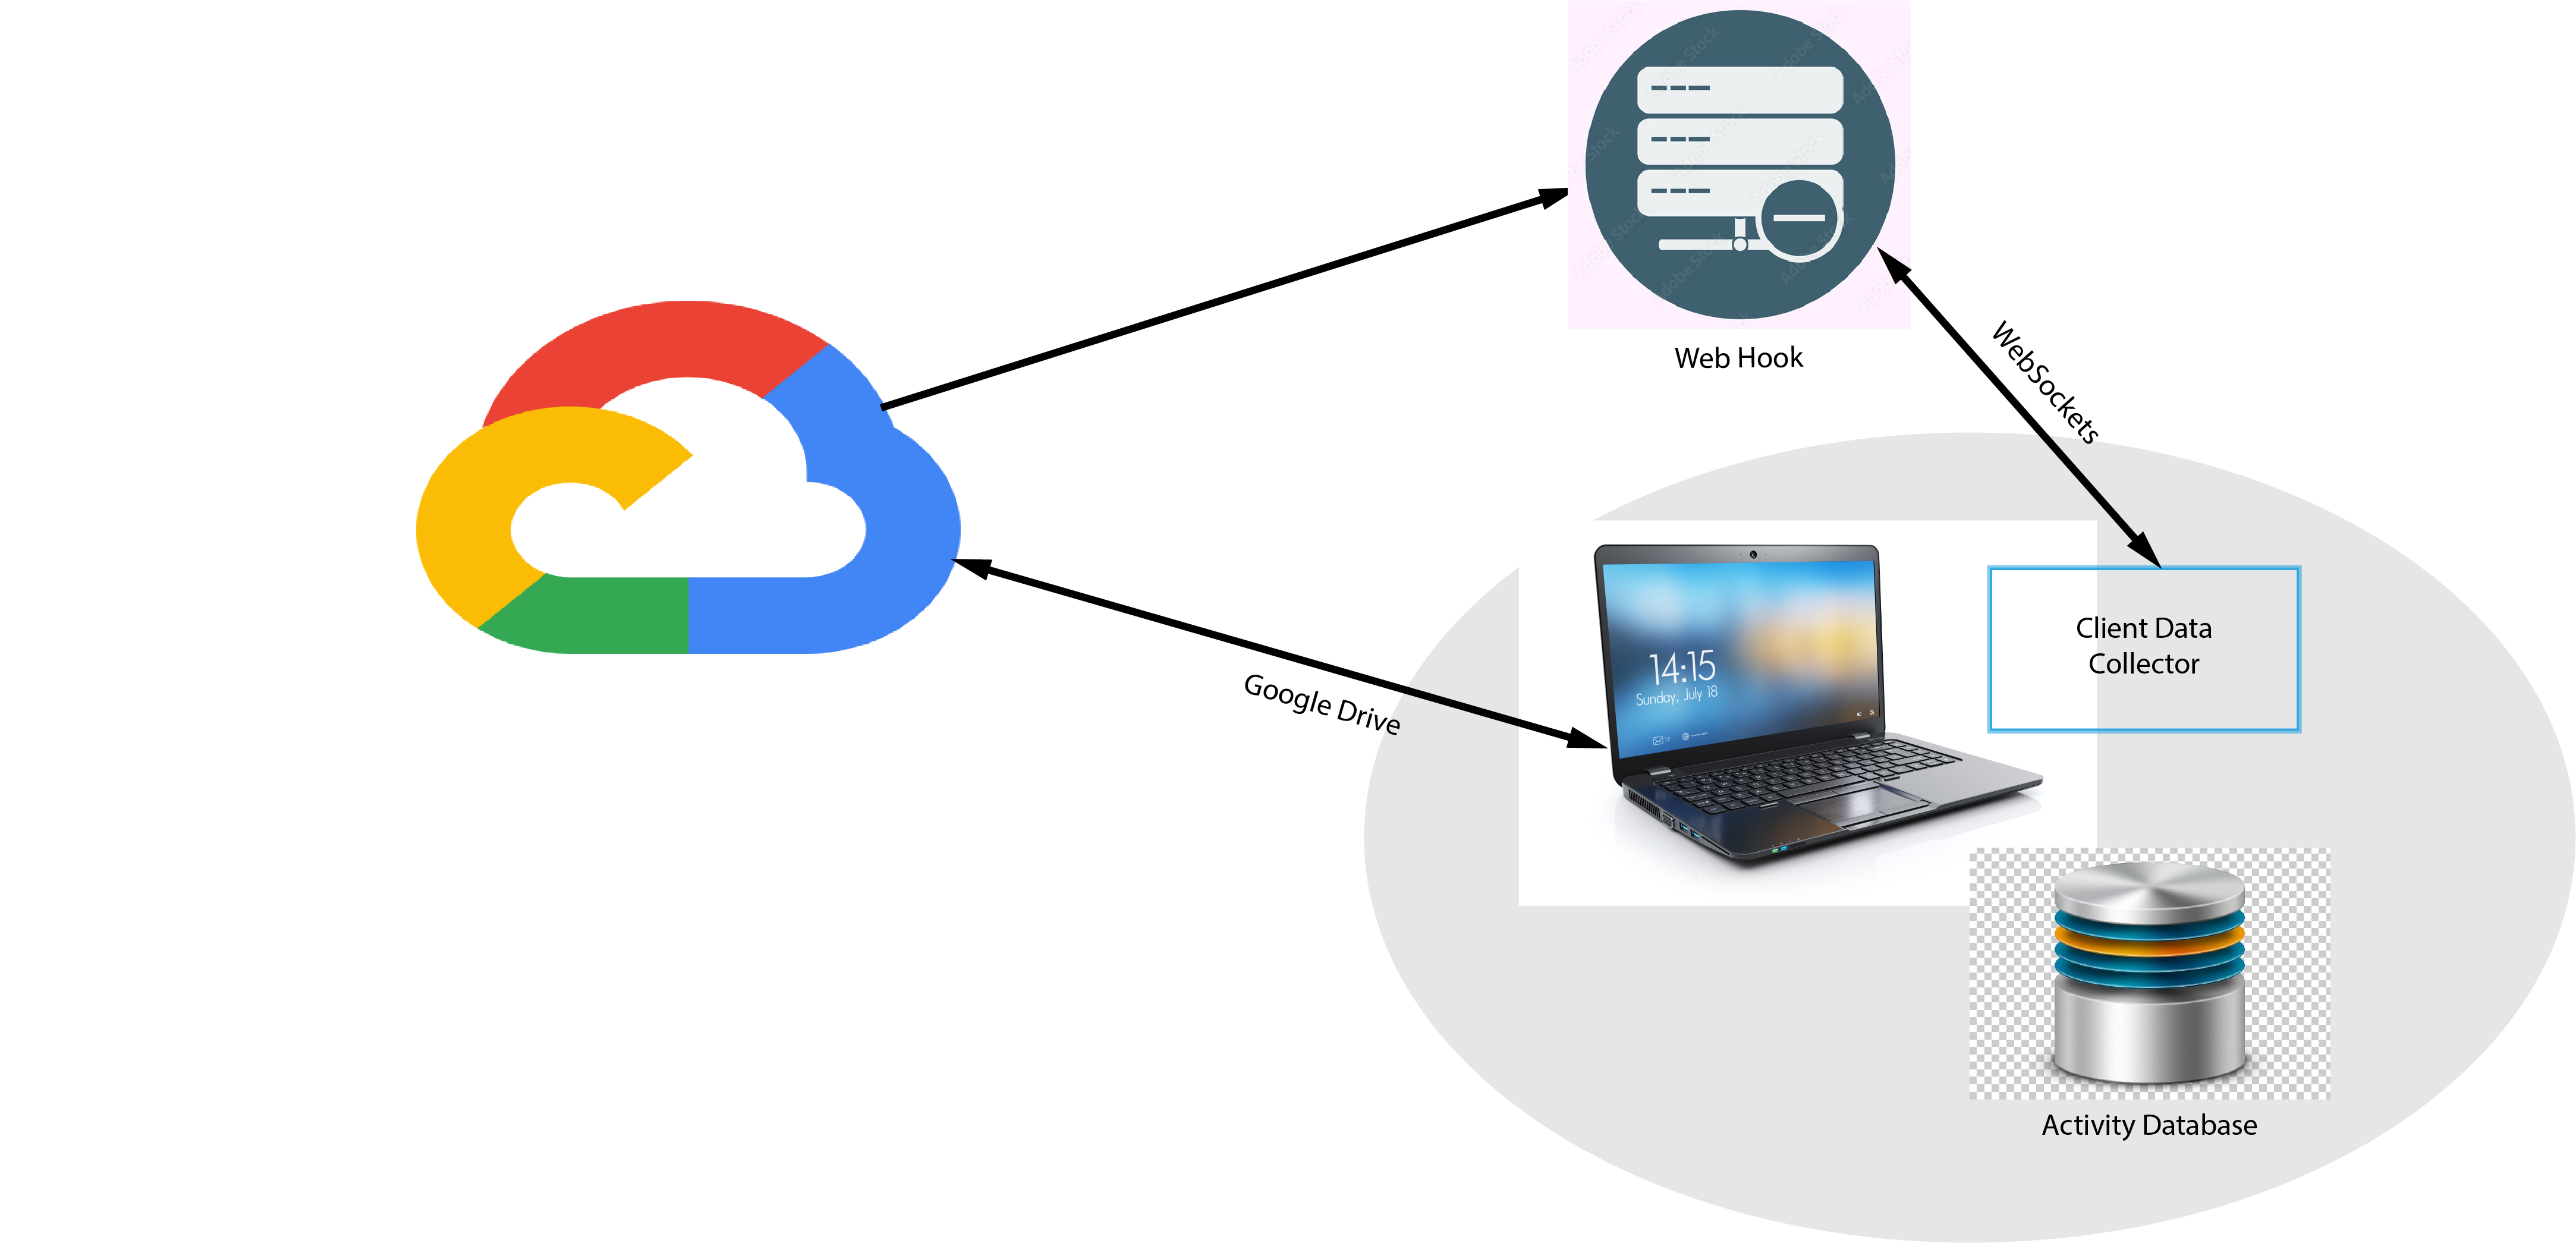
\includegraphics[width=0.45\textwidth]{figures/google-cloud-monitor.png}
    \end{tabular}
\end{figure}

For this work we chose to support Windows 11.  We monitored the system drive
using the Update Sequence Number (USN) Journal support provided by the NTFS File
system~\cite{huang2012research}.  This system provides a curated view of file
system activity on drives where the USN journal has been enabled. By default the
USN journal is enabled on the system drive and may be optionally enabled on
other drives.  This is a publicly documented API, has good performance, and
provides a curated level of information that provides benefit without being
``too broad.''

Similarly, we used a standard Dropbox installation (Version 154.4.5353).
Because Dropbox has an active agent on the local computer, we were able to
monitor changes made to the Dropbox contents via a public API that Dropbox
documents. \tm{Add reference to the API.}

Google Drive differs from Dropbox in that it does not rely upon a local agent on
the computer system.  Thus, we needed to construct a separate agent that
utilizes credentials and a callback registration mechanism so that Google Drive
will send notifications of events to the external service.  We show a simple
diagram of this arrangement in Figure \ref{fig:google-web-hook}. The Google
Drive Web API is a publicly documented API provided by Google.  The API between
the Web Hook and the local system on which we are storing activity information
is technically private. Our implementation of this was simple and merely used an
authenticated channel from the client to the Web Hook service on which to
receive notifications relayed from Google Drive via the Web Hook service.

\subsection{Considerations}

In my analysis of these various activity data sources, I have observed that:

\begin{itemize}
    \item It is broadly useful to have \emph{curation} over the data source.
    One of the challenges of reading from a ``fire hose'' is that the
    ``signal-to-noise'' ratio can be low.  Instead, the emphasis should be on
    capturing discrete events that are useful.

    \item To use labels to identify the specifics of particular relationships
    and properties to capture information that is useful to
\end{itemize}

\subsection{Evaluation}

\section{Storage}
\label{sec:storage}

A ``labeled property graph'' includes:

\begin{description}
    \item[node] --- in traditional mathematical graph descriptions this is the
    \emph{vertex}.  For my work this corresponds to a digital object, such as a
    file in a file system, a value in a key/value store, etc. Nodes within my/
    system have \emph{structure} because it must codify ``where'' the actual
    digital object is located in addition to the other information needed.  For
    practical purposes I think of the ``location'' as being a uniform resource
    identifier (\href{https://datatracker.ietf.org/doc/html/rfc8820}{URI}.)  The
    benefit of this paradigm is that it relies upon an existing standard for
    identifying objects, which is sufficient for my work.

    \item[relationship] --- in traditional mathematical graph descriptions this
    is the \emph{edge} that connects a pair of vertices.

    \item[identifier] --- this identifies the graph element (node or relationship).

    \item[label] --- this is a descriptive property related to the node or
    relationship.  For example, a label might identify that a node is a
    \emph{file} versus a \emph{value} in a key/value store.  Similarly, a label
    associated with a relationship would establish \emph{what} type of
    relationship this represents, such as a \emph{derived from} or a
    \emph{contained by} relationship.

    \item[property] --- this is essentially a key/value pair, where the key
    represents the property and the value represents the data associated with
    that property.  My goal is to permit some structure to a property, so that
    it may have a version associated with it, permitting more flexible upgrades
    to the format of the data.

\end{description}

I choose this model because it best fits the data I propose collecting, where
activity information is a type of \emph{node} and the associations between nodes
for storage elements and nodes for activity can form a relationship.

Since my goal is to find associations via contextual information, my work
describes both activity \emph{events} and activity \emph{contexts}.  An activity
\emph{event} is a node that an activity provider inserts to represent an
activity.  An activity \emph{context} is created on demand and forms a
relationship with some set of activity events.

Thus, the expectation is that we can retrieve the most recent instance of an
activity event of interest (where I leave defining \emph{of interest} to be
determined.)  For a simple demonstration, it likely makes sense to simply have a
list of the ``most recently added'' instance for each activity provider and
simply form the activity context by associating it.  As the number of activity
providers increases, further work will likely be needed to enable scaling.

Thus, an \emph{activity context} can be associated with other objects.  This
will permit us to subsequently examine the context of operations that were
ongoing at the time of interesting events.

This leads to a number of interesting questions to explore:

\begin{itemize}
    \item Does it make sense to maintain temporal relationships in this fashion;
    in other words, does the newest activity context point back to the previous
    activity context, or do the activity events point back to the older activity
    event?

    \item Should an activity context be something added implicitly (e.g., each
    time one creates a \emph{data} node, should the system automatically
    associate an activity context with it,) or explicitly (e.g., only when
    performed by an external agent.)

    \item How do we garbage collect this information?  That's not likely an
    important question to answer for prototypes, but it will become an important
    question as systems such as this emerge.

\end{itemize}

\subsection{Use Cases}

\subsection{Evaluation}

\section{Utilization}
\label{sec:utilization}

\subsection{Use Cases}

\subsection{Evaluation}

\section{Conclusion}

\tm{The idea that using behavioral advertising information could be beneficial
to file search would potentially be of interest to aggregation companies
because it would encourage use of these tools willingly: a ``free'' service
subsidized by advertising.}


\nocite{*}
\clearpage

\bibliographystyle{ACM-Reference-Format}
\bibliography{bib/indaleko.bib}

\end{document}

